% timetags (use of timetags for large-scale distributed microarchitectures)
%
\documentclass[10pt,dvips]{article}
\usepackage[english]{babel}
\usepackage{epsfig}
\usepackage{fancyheadings}
\usepackage[T1]{fontenc}
\usepackage[latin1]{inputenc}
%\usepackage{twocolumn}
%\usepackage{verbatim,moreverb,doublespace}
%\usepackage{rotate,lscape,dcolumn,array,rotating,latexsym}
%
%\input{epsf}
\textwidth 175mm
\textheight 225mm
\topmargin -15mm
\oddsidemargin 0mm
\evensidemargin 0mm
%
\pagestyle{empty}
%
\begin{document}
\parskip 3mm
%
%
\title{Coordination of Large-Scale Distributed 
Microarchitecture Using Time Tags}
%
\author{A. Uht\\
University of Rhode Island\\ uht@ele.uri.edu\\
% For a paper whose authors are all at the same institution,
% omit the following lines up until the closing ``}''.
% Additional authors and addresses can be added with ``\and'',
% just like the second author.
\and
D. Kaeli\\
Northeastern University\\
kaeli@ece.neu.edu\\
}
%
\maketitle
\thispagestyle{empty}
%
\begin{abstract}
Although studies suggest that significant amounts of instruction
level parallelism is present in many programs, significant progress
in extracting this parallelism has been very difficult.
In order to extract the inherent instruction level parallelism in
many programs, a large number of instructions need to be examined
and/or executed in parallel.  This necessitates a large microarchitecture
to accommodate a large amount of fine grained instruction execution.
We discuss a means by which a large distributed and scalable
microarchitecture can be controlled in a distributed way using
time tags.  Time tags serve as the basic coordinating mechanism
when large numbers of instructions are executing concurrently and
are also spatially distributed on silicon or multi-chip modules.
They enable the management of the architected program order as
it executes.  The basic idea, use, and management of time tags will
be discussed.  Finally, we present data showing how a modestly large
and microarchitecturally distributed machine performs using
the time tag based design approach.
\end{abstract}
%
\section{Introduction}
%
Studies into the limits of instruction level parallelism (ILP) have
been promising in that they have shown that there is parallelism within
many programs \cite{Lam92,Gon97}.  
Even programs that are quite sequential in nature and
not suitable for course grained parallelization exhibit parallelism due
to the control and data independent code block mixed throughout most
program codes \cite{Uht95}. 
Unfortunately, most of this fine grained
parallelism spans several basic blocks and the relatively small
instruction fetch windows of existing processor designs cannot span
the program instruction space necessary to begin to exploit this
parallelism.  Much larger numbers of instructions need to be both fetched
and executed concurrently in order to reveal the independent control
and data blocks and individual instructions that can provide higher
instructions per clock (IPC) to be realized.  A fundamental problem of
extracting this inherent parallelism is how to find it and execute it
concurrently while still managing the architectural program order that
is obviously necessary for proper program execution.
We also want to be able to manage the large-scale execution of
existing ISAs.  Further, there are advantages to finding
control and data independent code that are not available at compile time
(at least not without code profiling).  Therefor we want to make
maximum use of the hardware's ability to dynamically find, schedule,
and otherwise manage possible control and data independent instructions.

A much larger machine microarchitecture, capable of executing tens or
hundreds of instruction concurrently
is needed in order to exploit the fine grained parallelism in most sequential
programs.  The problem with large microarchitectures is the
competition for machine resources that have traditionally been
centralized.  These resources often include the register renaming logic, the
physical register file (including both architectural as well as renaming 
registers),
and the reorder buffer.  Other resources that are often centralized
in conventional microarchitectures are the execution units but those
do not present the same challenges for maintaining correct program order
as those resources that are associated with the architected registers
and the dependencies (control, register, and memory) that arise
from the instructions themselves.  The use of central resources
greatly hinders the scalability of any microarchitecture that
depends on them.
We present a microarchitecture that is able to scale to large sizes
through the
elimination of most conventional centralized microarchitectural components.
A new means to coordinate architected program order is necessary and
the use of time tags meets that need.  Time tags are used to maintain
and enforce correct program order for all flow dependencies whether
they be registers, memory values, or instruction control-flow predicates.
A much more detailed description of the general microarchitecture
assumed in this paper is presented in Uht et al \cite{Uht01}.

Section 2 will discuss a basic distributed microarchitecture that
achieves the above goals and how time tags are defined and used
to coordinate its execution flow.  
Section 3 discusses some of the differences between our envisioned
microarchitecture and existing ones.
Section 4 presents and discusses some simulation results using the proposed
microarchitecture.  Section 5 discusses some future work and
and section 6 summarizes the current work.

\section{Basic Distributed Microarchitecture Using Time Tags}

In order to achieve high IPCs in convention, single threaded, sequential
program codes many instructions need to be examined and executed
in parallel.  We desire that the span of instructions that might be
executed in parallel be on the order of at least tens and possibly hundreds
or thousands.  Unfortunately, exceedingly large numbers of instructions
in flight simultaneously puts an enormous burden on the access of
the physical register file (or files if they are partitioned in some way),
the architected register mapping function, and the reorder buffer 
needed for
management of the final committed program order.

\subsection{Active Stations and Execution Window}
To get around the typical problems of contention for centralized
machine resources, we have extended the idea of Tomasulo's reservation
station \cite{Tom67} to provide the basic building block for a distributed
microarchitecture.  Tomasulo's reservation station provided for the
simultaneous execution of different instructions over several
functional units.  This part of his scheme (already widely used) is
retained but extended to forward execution results to other spatially
separated and distributed reservation stations and execution units
rather than looping the results back to a common instruction issue unit
and update logic for the architected register file.  We also extend the idea
of the reservation station to allow for multiple executions (re-executions)
of the same instruction in the station.  We will keep an 
instruction in the station until it is retired (either committed or 
squashed).  
We call our adaptation of the reservation station the
\textit{Active Station}, abbreviated \textit{AS}.  
Some variations on this basic theme
will be discussed later.

Rather than lay our Active Stations out in silicon simply next to
function units that will execute the instructions issued to them,
we will lay them out in a two dimensional grid whereby sequentially
issued instructions will go to sequential ASes down a column of
the two dimensional grid of ASes.  The two dimensional
grid of ASes along with their interspersed execution units
is termed the \textit{Execution Window}.
In point of fact, the real
idea is to issue all of the instructions of a column of ASes simultaneously
in a single clock as much as possible.  How we can do this and
manage the typically troublesome control, register data, and memory
data dependencies is where the use of time tags enters in.

Fortunately, the basic operation of sequential programs provides
the very key to a large and distributed microarchitecture.
Since programs only need to forward instruction result operands into the
program ordered future, there is no real need to provide connectivity
for instruction result operands to be passed back to previously
executed (previous in program order) instructions.  This is the basic
idea of laying out the active stations in columns.  Result operands
from one instruction will flow forward to the next program instructions
that are in the ordered future of the program (whether those
instructions are speculative or not).  We will provide bus
interconnections (to be discussed later) that will allow for the
forwarding of instruction result operands from one active station to
those in the program ordered future.  Groups of active stations
that share execution resources are termed \textit{Sharing Groups}.

\subsection{Time Tags and Renaming}
Active stations are labeled with time tags.  A time tag is a small
integer that identifies a particular active station among the whole
set of them.  Active stations are labeled with time tags starting
from zero and incrementing up to one minus the total number of
active stations in a microarchitecture.  The time tag indicates
the program sequential order of the instructions that are issued
to active stations.  Time tags can be thought of as having two
component parts.  Since the active stations are laid out
in columns and rows, time tags can be viewed as having a column
part and a row part.  The column part is the high order bits of
the time tag integer.  The row part is what remains.

For illustrative purposes, we usually assign time tags, starting with the
value zero,
to active stations starting at the upper left corner of the two
dimensional grid of active stations and proceed to assign incremented
time tags first down the left-most column and continuing down the
next column to its right until all active stations are numbered.
The reader is again refered to Uht et al \cite{Uht01} for a more
detailed description of the arrangement of active stations within
the execution window and their possible interconnections.

Similarly to the conventional reservation station, operand results,
are broadcast forward for use by waiting instructions.
With active stations, all operands that are forwarded after the execution
of an instruction are also tagged with the time tag value of the
active station that originated the particular operand.
This tag will be used by subsequent active stations to determine if
the operand should be snarfed as an input operand that will trigger
the execution of its loaded instruction.

Essentially all values of any sort within the whole of the execution
window are tagged with time tags.
Since our microarchitecture can also allow for the concurrent
execution of multiple speculative paths of the current program,
we also introduce a path identification (path ID) number.
This path ID number
identifies the current path that an active station is executing an instruction
for.  
Path IDs are numbered (in our implementation) from zero and
incrementing to one minus the total number of possible paths
that the microarchitecture is designed to support.
Finally, path IDs are tagged to all operands in the execution window
along with the time tags.

The microarchitecture that we have devised requires the
forwarding of three types of operands.  These are register
operands, memory operands, and instruction predicate operands.
These are all tagged with time tags and path IDs that were associated
with the active stations that produces them.
Summarizing, the information 
actually broadcast from an active station to subsequent
ones in future program ordered time consists of :

\begin{itemize}
\item{a path ID}
\item{the time tag of the originating active station}
\item{the name of the architected operand}
\item{the actual data value for this operand}
\end{itemize}   

Figure \ref{fig:source} shows the registers inside an active
station for one of its input operands.  The 
\texttt{time-tag},
\texttt{address}, and
\texttt{value} registers are reloaded with new values on each snarf
while the
\texttt{path}, and
\texttt{AS time-tag} are only loaded when the active station is
issued an instruction.
The operand shown is typical for source registers, a source memory
operand, or an instruction execution predicate register.

\begin{figure}
\centering
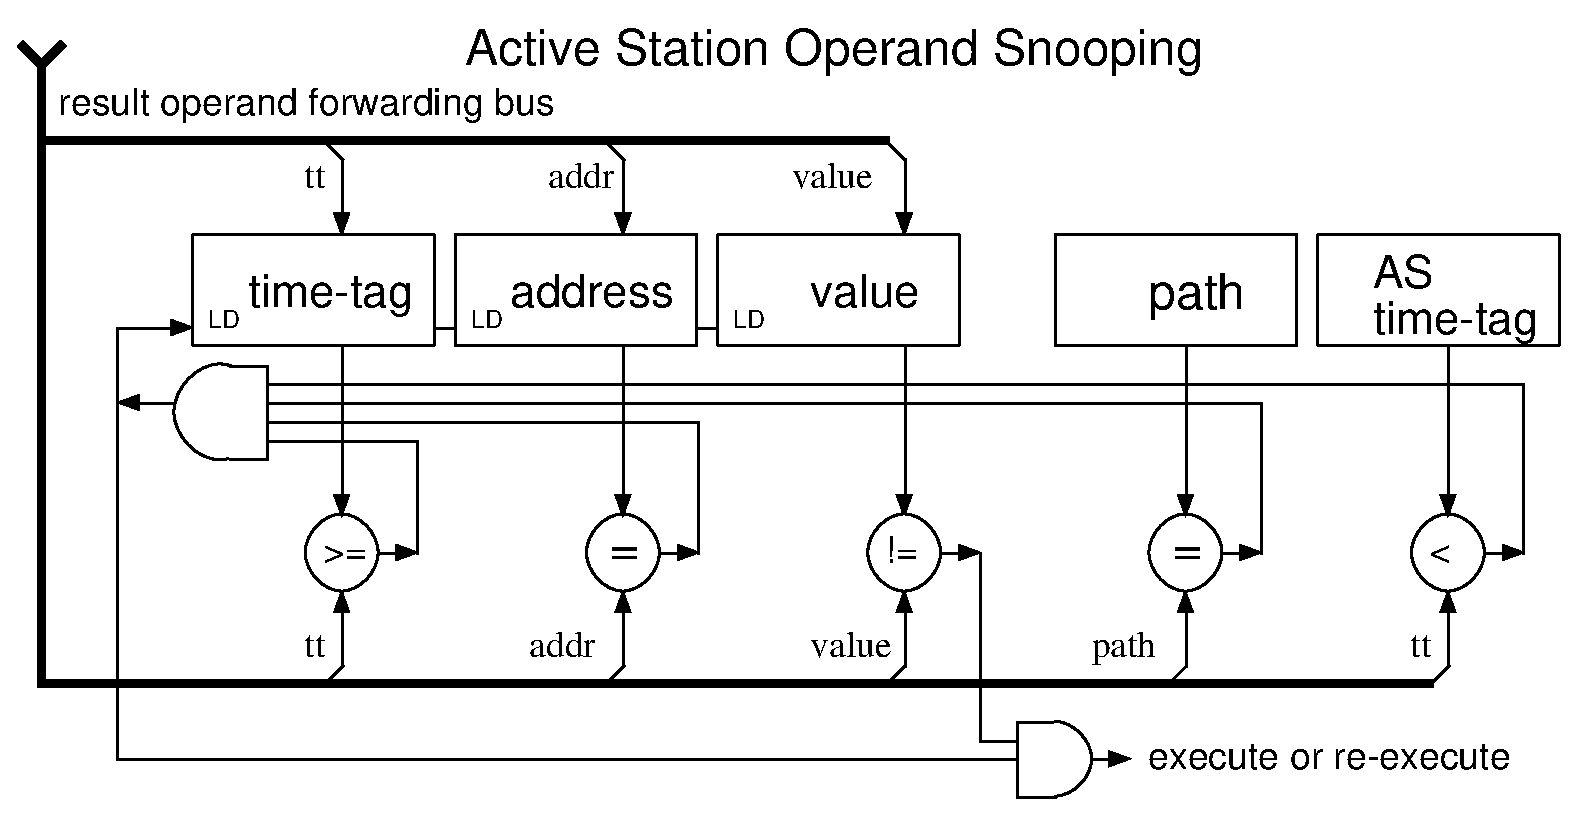
\epsfig{file=source.eps,width=5.8in}
\caption{{\em Active Station Source Operand.} The registers and snooping
operation of one of several possible source operands is shown.
Just one operand forwarding bus is shown being snooped but
typically several operand forwarding buses are snooped simultaneously.}
\label{fig:source}
\end{figure}

In the case of a register operand being forwarded, the name of the
operand is the address of the architected register.  For example
if the architected register in question is {\tt r6} then the
name of that operand would be the value 6.  If the operand
being forwarded is a memory operand, then the name of the operand
is simply its address (either a 32-bit address or a 64-bit address
depending on the machine ISA).  If the operand is a predicate,
then the name might be an internally derived value depending on
the way in which the automatic predication of instructions is
being done.  

The full name of an operand is a combination (a concatenation) of this
information described so far.  For example, the full name (the
{\tt rename} name) for a register operand would be :

{\tt path\_id:time\_tag:architected\_name}

For an active station executing an instruction for path ID 1
and having a time tag value of 26, and forwarding a result operand
for architected register \texttt{r6}, the corresponding name
of the operand in the name space of the whole machine would be :

{\tt 1:26:6}

This scheme effectively eliminates the need for rename registers
or other speculative registers as part of the reorder buffer.
The whole of the microarchitecture thus provides for the full renaming
of all operands thus avoiding all false dependencies.
There is no need to limit instruction issue or to limit speculative
instruction execution due to a limit on the number of non-architected
registers for holding those temporary results.

True flow dependencies are enforced through the continuous application of 
a snooping rule in each active station.  Each active station
will snoop all operands that are broadcast to it.  If the
path ID and the architected name of the operand match any of
its current input operands, the active station then checks
if the time tag value is less than its own assigned time tag
but is greater than or equal to the time tag value of the last
operand that it snarfed, if any.  If the snooped data value is
different than the input operand data value that the active
station already has, a re-execution of the instruction is initiated.
This simple rule will enforce
all proper flow dependencies while allowing for massive
concurrency of instruction executions.

\subsection{Result Forwarding Buses}
There are several choices for a suitable interconnection fabric between
the active stations.  This paper will not address (due to space) the
many and varied options that are available.  The purpose of the
interconnection fabric is to primarily forward instruction result
operands, tagged with their time tags, 
to those active stations in the program ordered future (those
active stations with higher valued time tags).  This means that one
basic requirement of the interconnection fabric is that it must be able
to transport operand results from any active stations in a column to
those active stations lower in the column and then to the remaining
active stations to the right of the current column starting again at
the top of the next column to the right.  So regardless of the number
and types of connections for interconnecting buses, the buses must
allow for the flow of operands from top left-most active station in the
grid, down the left-most columns of ASes, up to the top of the next and
repeating for all columns.

It must be noted at this point that operand result forwarding
bus connectivity is also needed (in a seemless way) from the bottom
right-most active station to the top left-most active station.
This is needed because assignment of time tags (as discussed so far)
is not going to remain static during the actual operation of the machine.
As columns of ASes retire and new columns are issued new instructions,
all of the time tags in the execution window are decremented by
an amount equal to the numbers of ASes in a column.  This corresponds
to decrementing the column part of each time tag in the whole of the
execution window by one.  Newly issued instructions will take on
time tags values corresponding to the right-most or highest numbered
column of ASes.  The new column that instructions are issued to used
to the column with the lowest numbered time tags, therefor bus
connectivity is provided in a circular fashion around all columns
in the execution window.

\section{Comparison With Conventional Approaches}

By developing a microarchitecture based around active stations
and the use of time tags to coordinate and enforce correct program
order, we eliminate the need for the severe contention that is necessarily
on either register scoreboards \cite{Thornton64} 
or the architected register files associated
with the use of reservation stations.  In those microarchitectures
that perform speculative execution (in the hardware), there is also
the need to access the reorder buffer, which becomes quite problematic
as the number of instructions being speculatively executed concurrently
approaches the hundreds or more.  Whether speculative instruction operand
results are stored in data registers within the reorder buffer or if the
results are stored in extra physical registers that hold both architected
and temporary values, the contention for the centralized resource is
the same.  In our microarchitecture, the whole of the set of active
stations form a giant reorder buffer or a sort.  The registers that
make up a reorder buffer in a conventional microarchitecture are
not eliminated entirely in the sense that we store the same speculative
information in a distributed way in each active station.  Similarly,
although the need for centralized rename registers is eliminated,
we are effectively storing the rename registers along with the
decoded instructions inside each active station.  Where the number of
physical registers in a convention machine may limit the amount of
outstanding speculated instructions, only the number of active stations
limits the amount of speculation that we can perform.

\section{Simulation Results}

We present results from simulations of a set of machine configurations
using the general microarchitecture and time tag tracking scheme described.

\subsection{Methodology}
The simulator is a recently built tool that shares some similarity
to Simple-Scalar \cite{Austin97} but was not based on it in any way.  
We execute
SpecInt-2000 and SpecInt-95 programs on simulated machines
that feature a MIPS-1 ISA along with the addition of some MIPS-2 and
MIPS-3 ISA instructions.  We are using the standard SGI Irix system
libraries so we needed some MIPS-2 and MIPS-3 instructions to accommodate
that.  All programs were compiled on an SGI machine under Irix 6.4 and
using the standard SGI compiler and linker.  The code was compiled with
standard optimization ({\tt -O}) for primarily the MIPS-1 ISA ({\tt -o32}).

\subsection{IPC Results and Discussion}
The data below are IPC results for various sized configurations of
a machine.  Two sets of data are provided.  The general features of
the machine simulated are 100% hit rates for L1 instruction cache,
a 1 cycle hit delay and 10 cycle miss penalty for the L1 data cache,
100\% hit in the L2 data cache, an operand forwarding delay of 1 clock
and a general bus delay of 1 clock.  The data cache is 32kB 2-way
set associative that is also 4-way interleaved on address bits 2 and 3.
Each of the machine configurations in Table \ref{tab:ipc} consist of three
numbers that give the rows of sharing groups, the number
of active station rows per sharing group, and the number of sharing
group column respectively.  The number of sharing group rows times the
number of active stations per sharing group is the total number of
active stations rows in a configuration.  These are all issued instructions
together in a single clock.

\makeatletter
%%%%%%%%%%%%%%%%%%%%%%%%%%%%%% LyX specific LaTeX commands.
\providecommand{\LyX}{L\kern-.1667em\lower.25em\hbox{Y}\kern-.125emX\@}
\makeatother

\begin{table}
\begin{center}
\caption{Benchmark IPC results for various machine sizes.}\label{tab:ipc}
\begin{tabular}{|c|c|c|c|c|c|c|}
\hline 
configuration&
4-4-4&
8-4-4&
8-4-8&
8-8-8&
16-8-4&
8-4-16\\
\hline
\hline 
bzip2&
2.7&
3.9&
4.3&
5.1&
4.5&
4.9\\
\hline 
parser&
2.6&
3.9&
4.8&
5.7&
4.4&
5.3\\
\hline 
gzip&
2.8&
4.0&
4.6&
5.8&
5.2&
5.6\\
\hline 
gap&
3.3&
4.9&
5.9&
6.5&
5.8&
6.0\\
\hline 
go&
2.9&
4.2&
5.4&
6.3&
4.8&
5.6\\
\hline 
harmonic mean&
2.8&
4.2&
4.9&
5.8&
4.9&
5.4\\
\hline
\end{tabular}
\end{center}
\end{table}

As can be seen from the data, the configuration of 8-8-8 provides
the best overall IPC for the configurations simulated.  This consists
of 64 active stations in each column with 8 columns.
Configuration 16-8-4 does not perform as well because it does not
have as many columns (only 4 as compared with 8 in the other configuration)
to hide the latencies of instruction execution.  Eight columns 
hides more instruction execution latency than four.  The 8-4-16
configuration performs poorly as compared with 8-8-8 because the height
of a column (the primary IPC multiplier) is only 32 and its extra
columns are not needed to hide more instruction execution latency.

\section{Future Work}

Much work remains to investigate numbers and type of interconnecting
buses, the strategies for operand forwarding, and the policies inside
the various bus repeater and operand filtering units.
Work also continues on fetching policies and heuristics and on
D-path spawning.

\section{Summary}

We have presented a new microarchitecture, extended from Tomasulo's
reservations stations, that uses time tags to coordinate and enforce
program order on large-scale out of order execution.
The use of time tags allows for the scalability of our microarchitecture
to sizes that can allow for hundreds of instructions (or more) to execute
concurrently.
Our results indicate that this general approach appears to be quite
promising as compared with the existing more conventional microarchitectural
approaches.  Some work on much larger machine configurations has already
suggested that achieving IPC numbers in the 10s on general integer
sequentially-oriented program codes is possible.

\bibliographystyle{latex8}
\bibliography{timetags}

\end{document}
%
%
